\section{Empirical Improvements}\label{sec:empirical}

% \anoteinline{Whenever we are measuring $\ell_2$-squared error, we should say indepdendnet noise (a.k.a. DP-SGD).}
% \agnote{I think we only do in 6.2, and we clal it "independent noise" primarily?}

We implement \CPTB{} by building on methods in the open-source \texttt{dp\_accounting} Python library \citep{pldlib}, and perform empirical studies of the amplification benefits from \MMCC{}.  PLD accounting for MoG mechanisms is currently open-sourced as part of the \texttt{dp\_accounting} library. We plan to open-source our implementation of \CPTB{} building on top of \texttt{dp\_accounting}. There are some challenges in the implementation which we discuss in \cref{sec:implementation}. For simplicity we use $\delta_1, \delta_2 = \delta/2$ in \CPTB{}.

\subsection{Binary tree mechanism amplification}
In this section, we show how the privacy guarantee of the binary tree mechanism empirically improves if we use sampling and \MMCC{}.

As a baseline, we fix a constant $c$, and consider the binary tree mechanism under a single-participation constraint, with $\sigma = c \sqrt{\log(n) + 1}$. By the analysis of the Gaussian mechanism, for all $n$ that are powers of 2, the binary tree mechanism with this choice of $\sigma$ under a single-participation constraint without amplification satisfies $(\epsilon, \delta)$-DP for the same $\epsilon, \delta$. In other words, as we increase $n$, the privacy guarantee of the unamplified mechanism remains fixed. Then, for the same $c$ and $n$ that are powers of 2, we use \CPTB{} to compute a privacy guarantee for the binary tree mechanism with subsampling probability $1/n$ and the same choice of $\sigma$.  By the analyses in Section~\ref{sec:ftrl}, we expect that with subsampling, the value of $\epsilon$ will decrease as $\Omega(\sqrt{\log n})$.

\begin{figure}
    \begin{subfigure}{.33\textwidth}
      \centering
      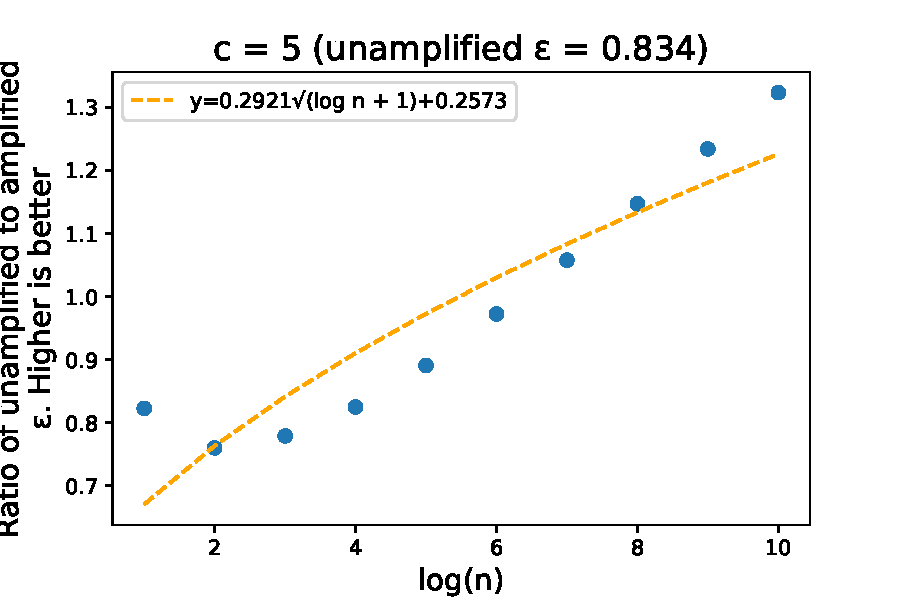
\includegraphics[width=.95\linewidth]{plots/binary_tree_c=5.pdf}
      \label{fig:btc=5}
    \end{subfigure}
    \begin{subfigure}{.33\textwidth}
      \centering
      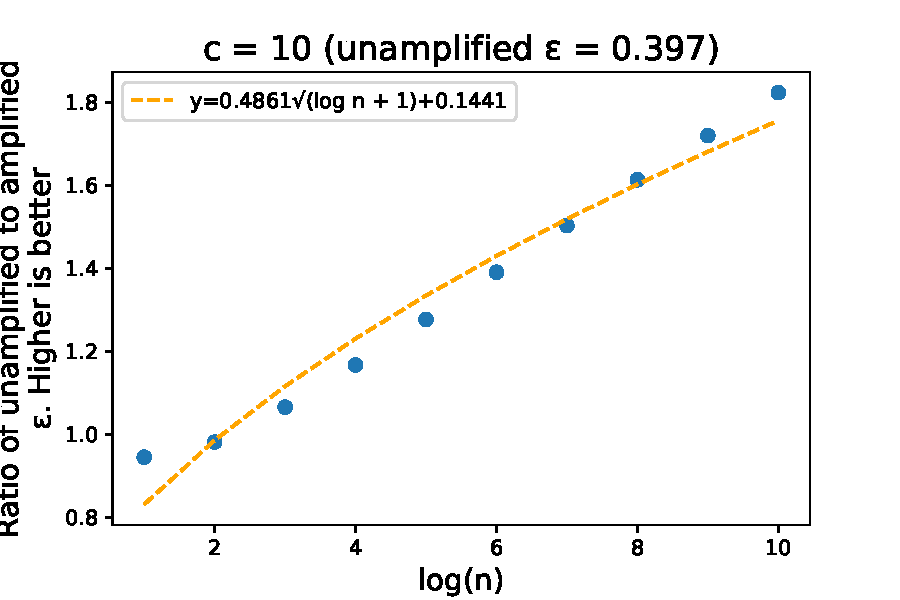
\includegraphics[width=.95\linewidth]{plots/binary_tree_c=10.pdf}
      \label{fig:btc=10}
    \end{subfigure}
    \begin{subfigure}{.33\textwidth}
      \centering
      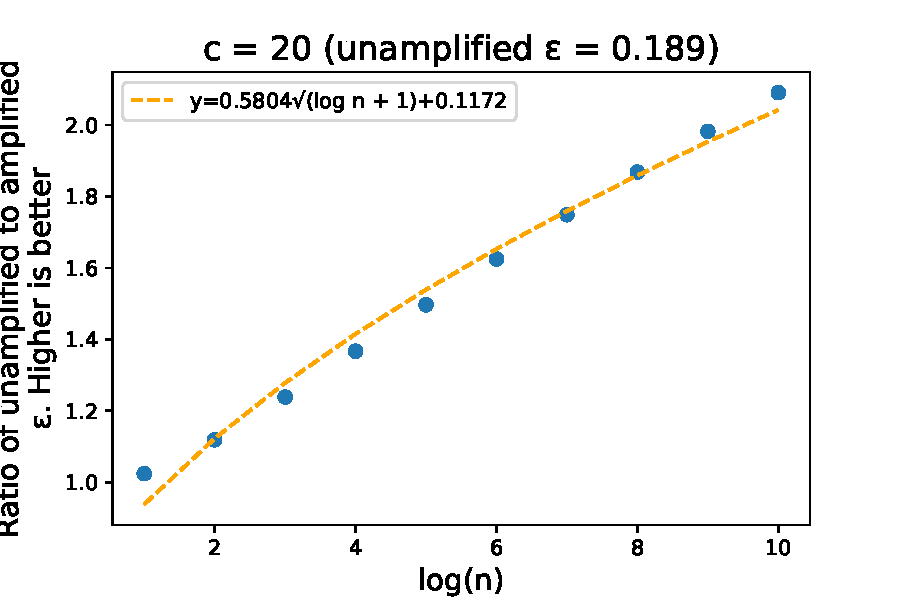
\includegraphics[width=.95\linewidth]{plots/binary_tree_c=20.pdf}
      \label{fig:btc=20}
    \end{subfigure}
\caption{\label{fig:tree-empirical}\textbf{Multiplicative improvement of our amplification analysis (roughly) matches $\sqrt{\log(n) + 1}$.} A higher ratio ($>1$) indicates amplification is better. We plot $n = 2^i, i \in \{1, 2, \ldots, 10\}$ with $\sigma = c \sqrt{\log(n) + 1}$ so $\epsilon$ is fixed for unamplified single-participation. $\delta = 10^{-6}$.}
\end{figure}

In \cref{fig:tree-empirical}, we observe that empirical improvement in $\epsilon$ due to amplification is roughly proportional to $\sqrt{\log(n) + 1}$.
%
% In~\cref{fig:tree-empirical}, we plot the ratio of the $\epsilon$ value computed for the unamplified binary tree mechanism, divided by the $\epsilon$ value computed for the binary tree mechanism with subsampling. In each plot, we fix $\delta = 10^{-6}$ and use a fixed value of $c$ in $\{5, 10, 20\}$, and plot the ratio for each $n$ that is a power of 2 between $2$ and $1024$. We also compute and plot the solution to least-squares linear regression for these ratios as a function of $\sqrt{\log(n) + 1}$. 
%
We also observe two improvements as $c$ (i.e., $\sigma$) increases. First, the multiplicative improvement in $\epsilon$ increases; second, empirical improvements better match a linear fit to $\sqrt{\log(n) + 1}$. Both these improvements are explained by the fact that (as discussed in \cref{sec:cptb}) as $\sigma \rightarrow \infty$, \MMCC{} reports a tighter $\epsilon$.

\subsection{Amplification for optimal continual counting}

\cite{HU22, HUU23} showed that a post-processing of the matrix mechanism using the following lower-triangular matrix achieves $1+o(1)$ times the optimal $\ell_2^2$ error for prefix sums (without amplification): $\bfC_{i,j} = f(i-j)$, where $f$ is defined as

\[f(k) = \left\{
\begin{array}{lr}
        0, & \text{for } k < 0\\
        1, & \text{for } k = 0\\
        f(k-1) \cdot \left(1 - \frac{1}{2k}\right), & \text{for } k > 0
\end{array}
\right..\]

Similarly to the binary tree mechanism, we will consider the unamplified single-participation setting as a baseline. In this case, the sensitivity of this matrix mechanism is $\ltwo{\bfC \bfe_1}$, i.e. the $\ell_2$-norm of the first column of $\bfC$. So again, setting $\sigma = c \ltwo{\bfC \bfe_1}$ results in a fixed $\epsilon$ for a fixed $\delta$. Our comparison will be applying the same matrix mechanism with subsampling probability $1/n$ and the same choice of $\sigma$. 

\begin{figure}
    \begin{subfigure}{.33\textwidth}
      \centering
      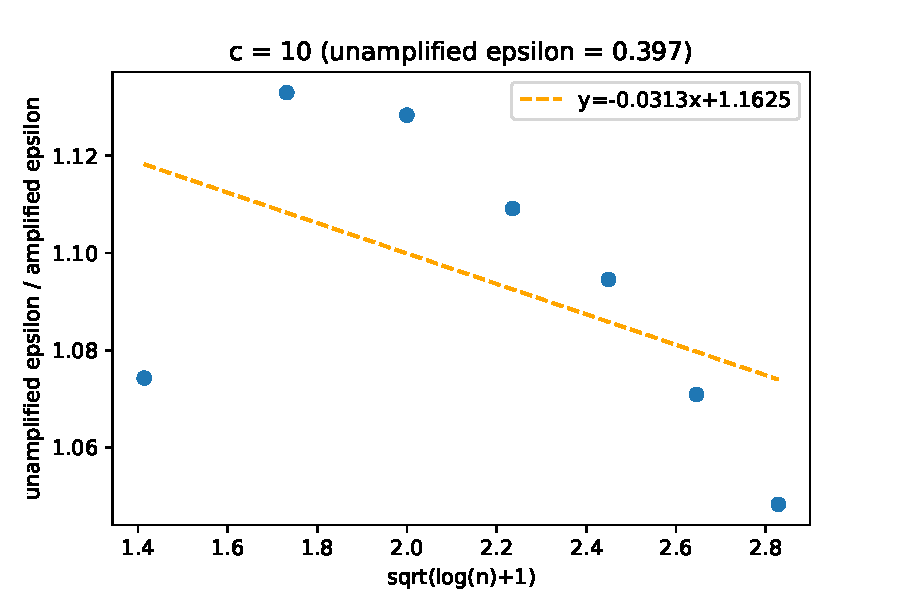
\includegraphics[width=.95\linewidth]{plots/continual_obs_c=10.pdf}
      \label{fig:ccc=10}
    \end{subfigure}
    \begin{subfigure}{.33\textwidth}
      \centering
      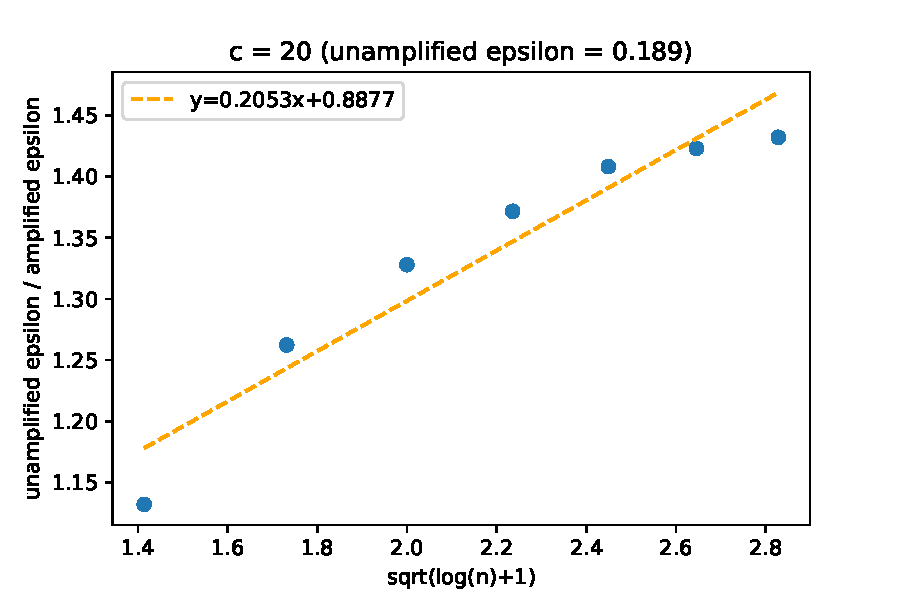
\includegraphics[width=.95\linewidth]{plots/continual_obs_c=20.pdf}
      \label{fig:ccc=20}
    \end{subfigure}
    \begin{subfigure}{.33\textwidth}
      \centering
      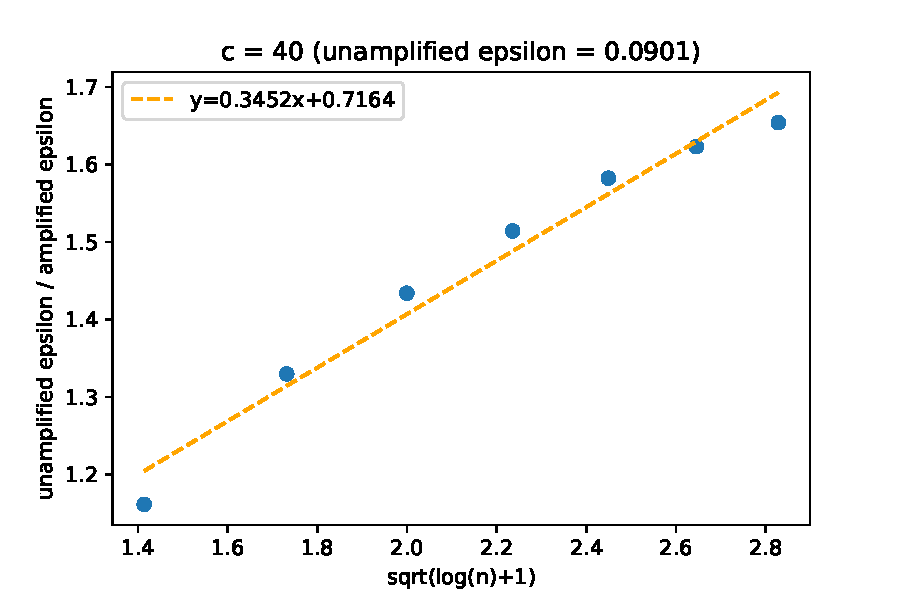
\includegraphics[width=.95\linewidth]{plots/continual_obs_c=40.pdf}
      \label{fig:ccc=40}
    \end{subfigure}
\caption{Plot of multiplicative improvement in $\epsilon$ for the optimal continual counting matrix mechanism as a function of $\sqrt{\log(n) + 1} \approx \ltwo{\bfC \bfe_1}$.  We plot $n = 2^i, i \in \{1, 2, \ldots, 7\}$. We use $\sigma = c \ltwo{\bfC \bfe_i}$, so the $\epsilon$ value in the unamplified single-participation setting is fixed. All $\epsilon$ are for $\delta = 10^{-6}$.}
\label{fig:cc-empirical}
\end{figure}

In~\cref{fig:cc-empirical}, we reproduce the plots in~\cref{fig:tree-empirical} but for this matrix mechanism instead of the binary tree mechanism. The $\ell_2$-norm of the columns of this matrix asymptotically are $\Theta(\sqrt{\log n})$; because of this, and to make a direct comparison to the binary tree mechanism easier, we use $\sqrt{\log(n) + 1}$ as the x-axis and plot the least squares linear regression. Because the columns of this matrix are less orthogonal than those of the matrix for the binary tree mechanism, there is less benefit from amplification in this setting than the binary tree mechanism setting, so we use a larger range of values $c \in \{10, 20, 40\}$ for the noise multiplier to better demonstrate the behavior of the improvement in $\epsilon$.

For sufficiently large $\sigma$, the improvement in $\epsilon$ due to the amplification analysis is again roughly proportional to $\sqrt{\log (n) + 1}$. For the same reasons as for the binary tree mechanism, the fit of the linear regression is better as $\sigma$ increases: here, because the columns of this matrix are less orthogonal on average, a larger value of $c$ is needed for the fit to improve. Here, the constant multiplier in the improvement is smaller; this makes sense as these matrices improve on the error of the binary tree mechanism by a constant, and thus the amount by which we can improve the privacy analysis of this matrix mechanism without violating lower bounds is smaller than for the binary tree mechanism. 

% \subsection{Amplified banded DP-MF}

% In \cite{BandedMF}, the authors consider using $b$-banded matrices (matrices where $\bfC_{i,j} = 0$ if $i-j \geq b$) in the matrix mechanism in the context of designing algorithms for private optimization with lower variance than DP-SGD. They achieve amplification for these matrices using a slightly different sampling scheme than what we consider in this paper: They partition the dataset into $b$ subsets, and in round $i$ sample examples from the $i \pmod b$-th subset to compute $\bfx_i$. If we want to use an expected fraction $p$ of examples from the entire dataset in each round, then our sampling probability when sampling from each subset should be $bp$. So, they effectively show banded matrices satisfy the privacy guarantees of composing $n/b$ subsampled Gaussians with sampling probability $bp$ and sensitivity $\max_i \ltwo{\bfC \bfe_i}$. 

% We have discussed the qualitative advantages of our result over this amplification result in the introduction; here we provide a quantitative comparison. We generate the optimal 64-by-64 $b$-banded matrix for $b \in \{2, 4, 8\}$ using the procedure detailed in \cite{BandedMF}. 
% %\anoteinline{How did we get this code? Does it break anonymity?} 
% We also take the 64-by-64 version of the matrix of \cite{HU22} considered in the previous section, and zero out all entries $(i, j)$ such that $i - j \geq b$ to make them $b$-banded. We then compute $\epsilon$ using \CPTB{} as well as using the analysis in \cite{BandedMF}, for $\sigma \in \{10, 20, 40\}$ as well as sampling probability $p \in \{1/64, 2/64, 4/64, 8/64\}$; for the approach of \cite{BandedMF}, we use sampling probability $bp$ instead. In \cref{fig:bandedratios} we give the ratios of the epsilons computed this way.

% \begin{figure}
% \begin{tabular}{lll}
%     \cite{BandedMF} & & \\
%     \begin{subfigure}{.33\textwidth}
%       \centering
%       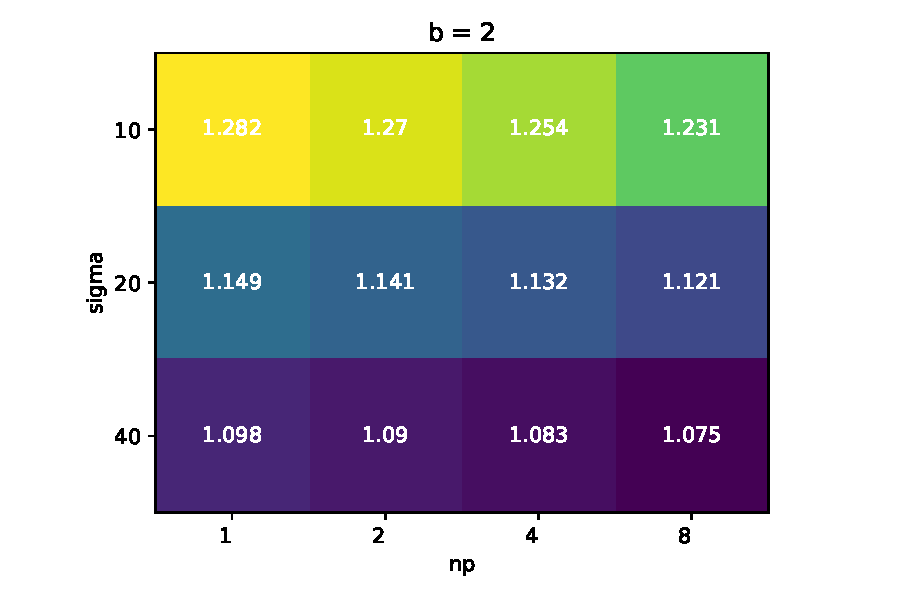
\includegraphics[width=\linewidth,trim={1 0 0 1}]{plots/banded_ratios_2.pdf}
%       \label{fig:br2}
%     \end{subfigure}
%     &
%     \begin{subfigure}{.33\textwidth}
%       \centering
%       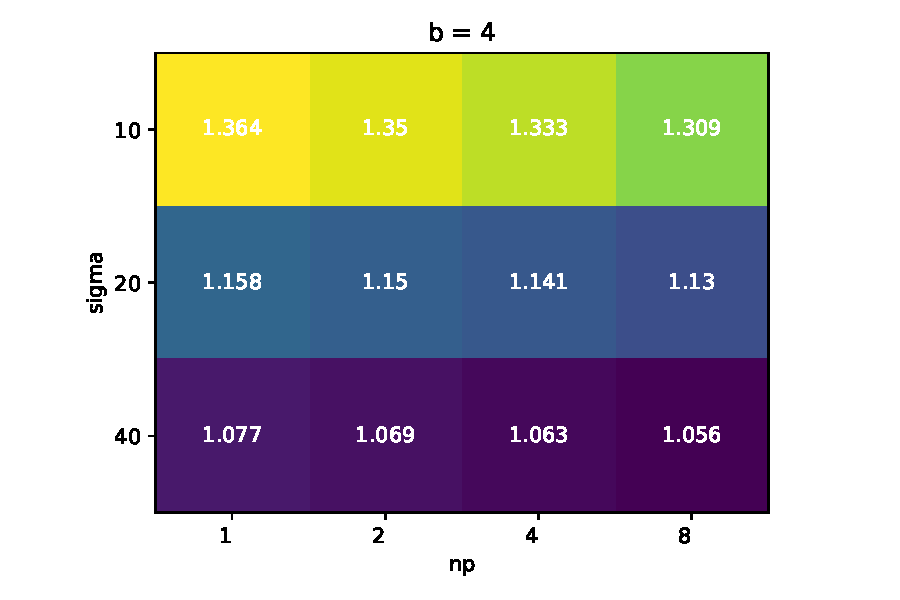
\includegraphics[width=\linewidth,trim={1 0 0 1}]{plots/banded_ratios_4.pdf}
%       \label{fig:br4}
%     \end{subfigure}
%     &
%     \begin{subfigure}{.33\textwidth}
%       \centering
%       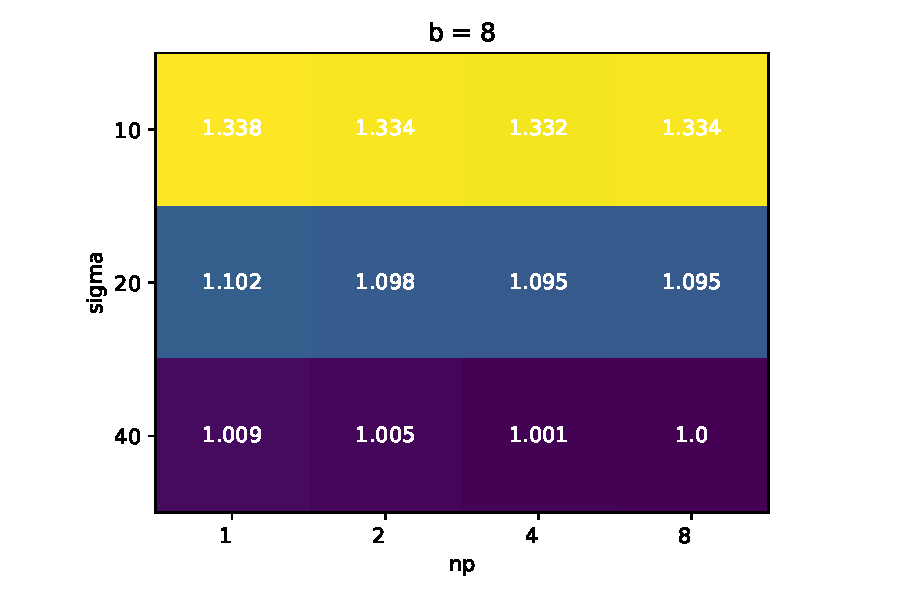
\includegraphics[width=\linewidth,trim={1 0 0 1}]{plots/banded_ratios_8.pdf}
%       \label{fig:br8}
%     \end{subfigure}
%      \\
%     \cite{HU22} & & \\
%     \begin{subfigure}{.33\textwidth}
%       \centering
%       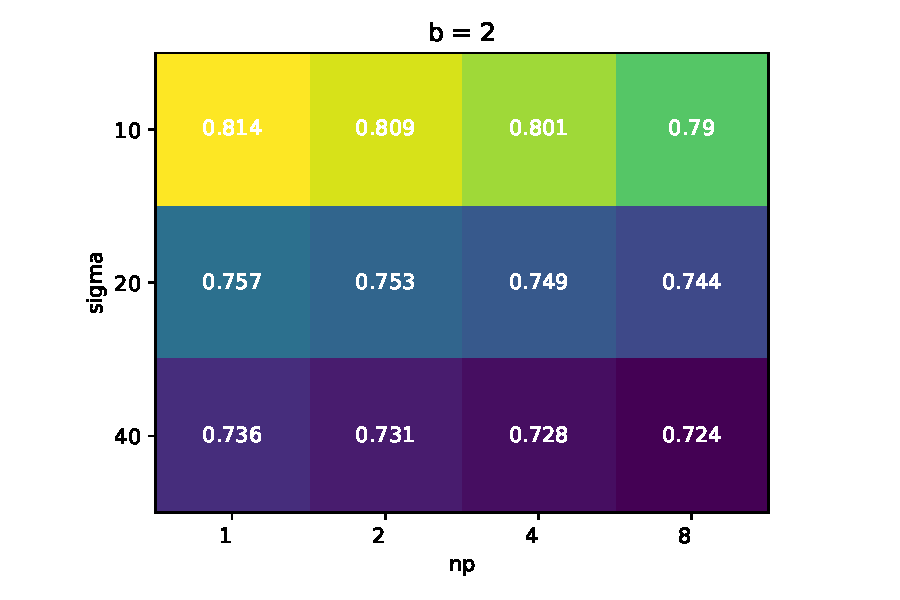
\includegraphics[width=\linewidth,trim={1 0 0 1}]{plots/fhu_banded_ratios_2.pdf}
%       \label{fig:br2-hu}
%     \end{subfigure}
%     &
%     \begin{subfigure}{.33\textwidth}
%       \centering
%       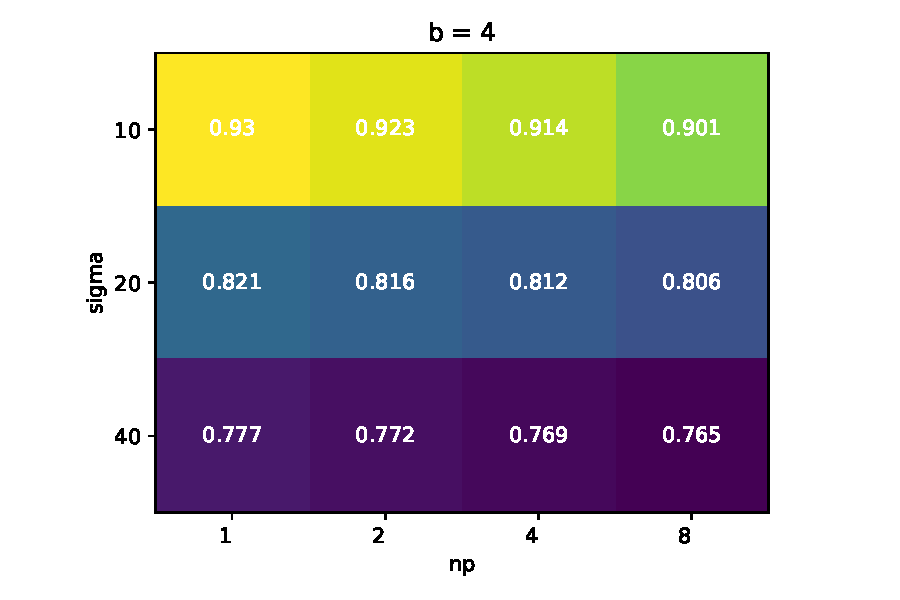
\includegraphics[width=\linewidth,trim={1 0 0 1}]{plots/fhu_banded_ratios_4.pdf}
%       \label{fig:br4-hu}
%     \end{subfigure}
%     &
%     \begin{subfigure}{.33\textwidth}
%       \centering
%       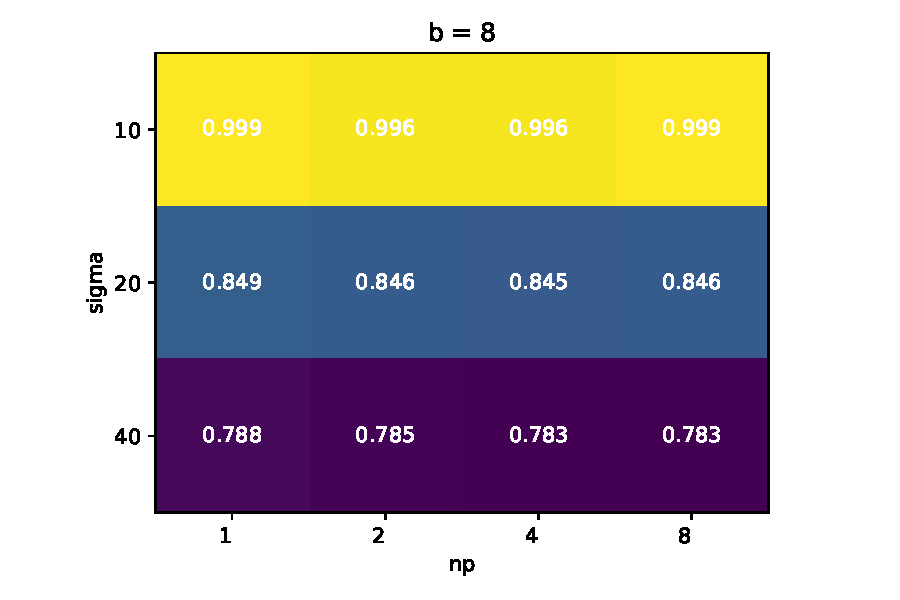
\includegraphics[width=\linewidth,trim={1 0 0 1}]{plots/fhu_banded_ratios_8.pdf}
%       \label{fig:br8-hu}
%     \end{subfigure}
% \end{tabular}
% \caption{Plot of multiplicative improvement in $\epsilon$ for banded matrices computed in \cite{BandedMF}. For each type of matrix and combination of $b, \sigma, p$ we list the ratio of $\epsilon$ computed using our approach divided by $\epsilon$ computed using the approach in \cite{BandedMF}, i.e. a ratio $< 1$ represents an improvement from our result.}
% \label{fig:bandedratios}
% \end{figure}

% \anoteinline{For the comparison to~\cite{BandedMF}, we are making contrasting claims to that in the introduction. We are saying that ours is better in the intro, but here we are not being able to provide a conclusive evidence.}

% For the matrices generated by \cite{BandedMF}, \CPTB{} reports worse than epsilons than the approach in \cite{BandedMF}. On the other hand, for the truncated versions of the matrices of \cite{HU22}, we see improvements in $\epsilon$ from \CPTB{}.
% We conjecture this is because of the structure of the matrices generated by \cite{BandedMF}, which can be visualized in \cref{fig:banded-matrices}. In general, we expect that doing i.i.d sampling every round gets better privacy amplification as columns become closer to orthogonal, as this near-orthogonality corresponds to smaller correlation between rows of $\bfC \bfx$. However, \cite{BandedMF} optimize their matrices under only a bounded column norm constraint, i.e. with no consideration for the dot product of adjacent columns. 
% In particular, looking at \cref{fig:banded-matrices} we see the columns are not strictly non-increasing, which lends to columns having larger dot products. So the improvements for these matrices due to using i.i.d. sampling instead of the sampling scheme of \cite{BandedMF} are limited. Combined with the slack in the analysis of \CPTB{}, this leads to worse $\epsilon$ computations. On the other hand, the matrices of \cite{HU22} have decreasing columns, i.e. have columns that are closer to orthogonal. So, these can benefit more from i.i.d. sampling every round than the matrices in \cref{fig:banded-matrices}, enough to make up for the slack in \CPTB{}.

% \anoteinline{I am not sure this detailed discussion on why we are sub-par with~\cite{BandedMF} is necessary here. We should move the main points to a footnote. The reviewers may not take this positively.}

% \begin{figure}
%     \begin{subfigure}{.33\textwidth}
%       \centering
%       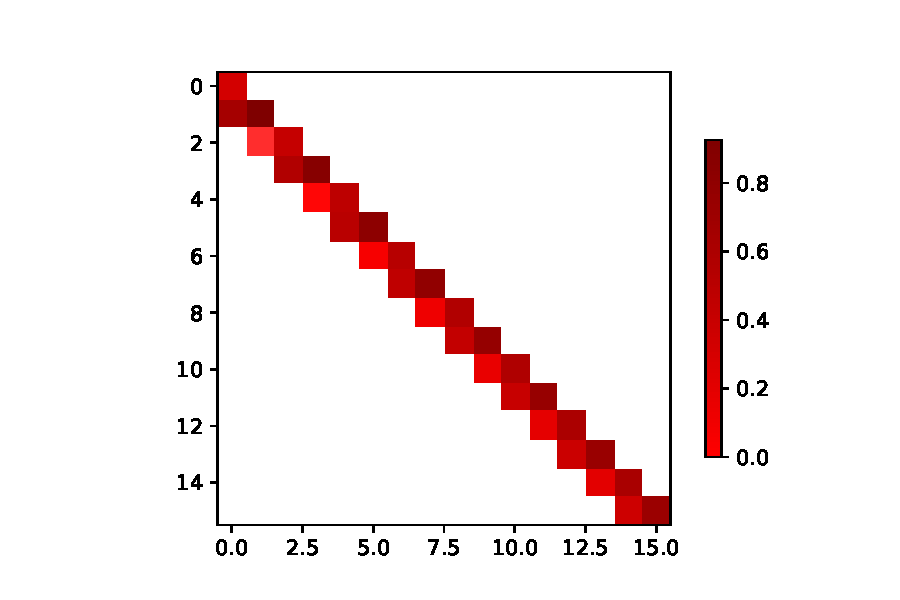
\includegraphics[width=.95\linewidth]{plots/banded-matrix-2.pdf}
%       \label{fig:16-by-16-2}
%     \end{subfigure}
%     \begin{subfigure}{.33\textwidth}
%       \centering
%       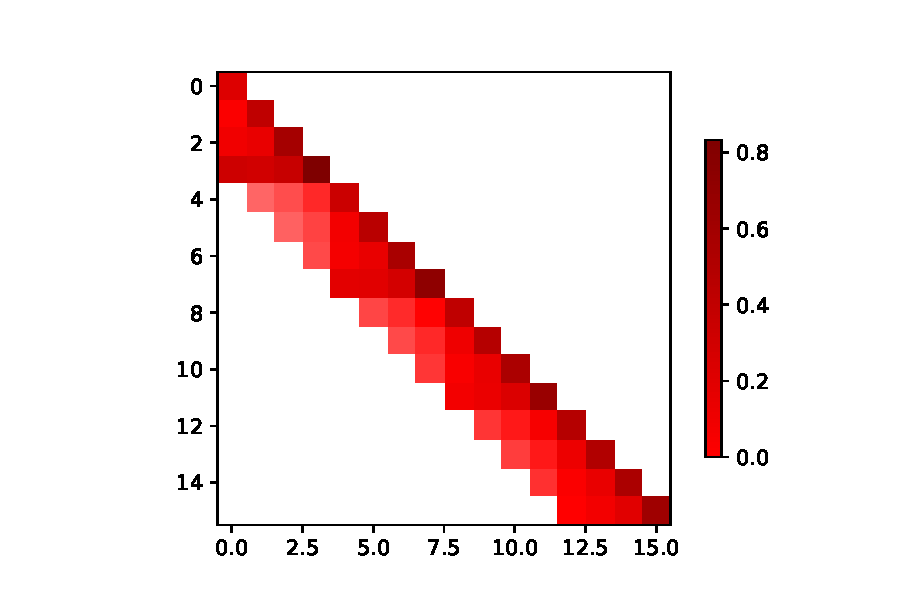
\includegraphics[width=.95\linewidth]{plots/banded-matrix-4.pdf}
%       \label{fig:16-by-16-4}
%     \end{subfigure}
%     \begin{subfigure}{.33\textwidth}
%       \centering
%       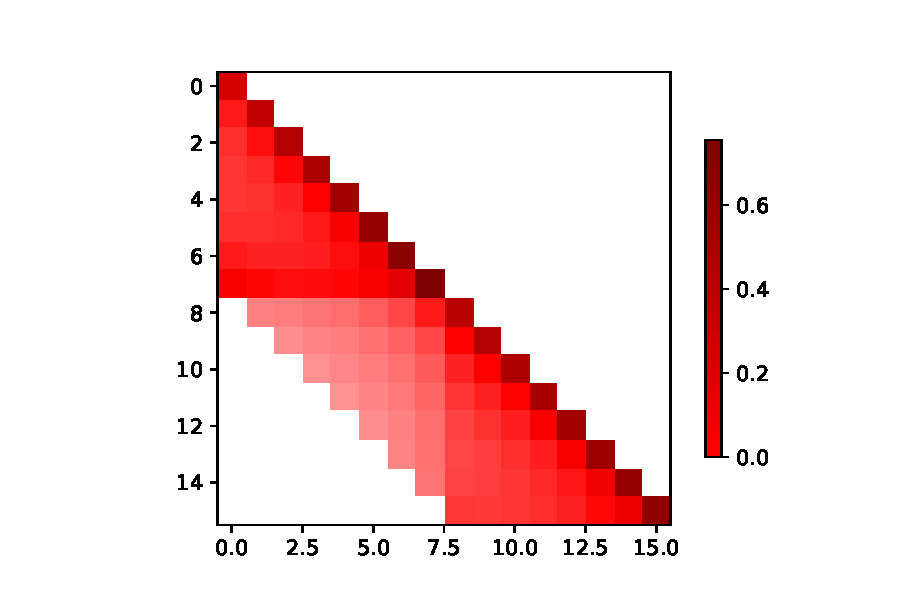
\includegraphics[width=.95\linewidth]{plots/banded-matrix-8.pdf}
%       \label{fig:16-by-16-8}
%     \end{subfigure}
% \caption{The top-left 16-by-16 submatrix of the matrices we generated using code of \cite{BandedMF}.}
% \label{fig:banded-matrices}
% \end{figure}

\subsection{Learning Experiments with Binary-Tree-DP-FTRL}
A motivating reason for us to study matrix mechanisms is that the analysis of~\citet{kairouz2021practical} has a suboptimal scaling in the amount of noise added, which manifests in their experiments with DP machine learning. We reproduce the centralized DP training on CIFAR-10 from~\citet{MEMF}, including model architecture, tuning setup, hyperparameter choices, and optimizations to the tree aggregation mechanism for ML; we use these as our baseline results.

In \cref{fig:improve-banded}, we re-analyze the baseline using \MMCC{} and show significant improvements in privacy-utility tradeoffs for DP-FTRL via binary trees. In particular, we observe that these benefits become larger as $\epsilon$ becomes small. Note that these improvements are entirely ``post-hoc,'' i.e. the algorithm is the same, but with a better privacy analysis.

\begin{figure}
\centering
\begin{minipage}{.45\textwidth}
    \centering
    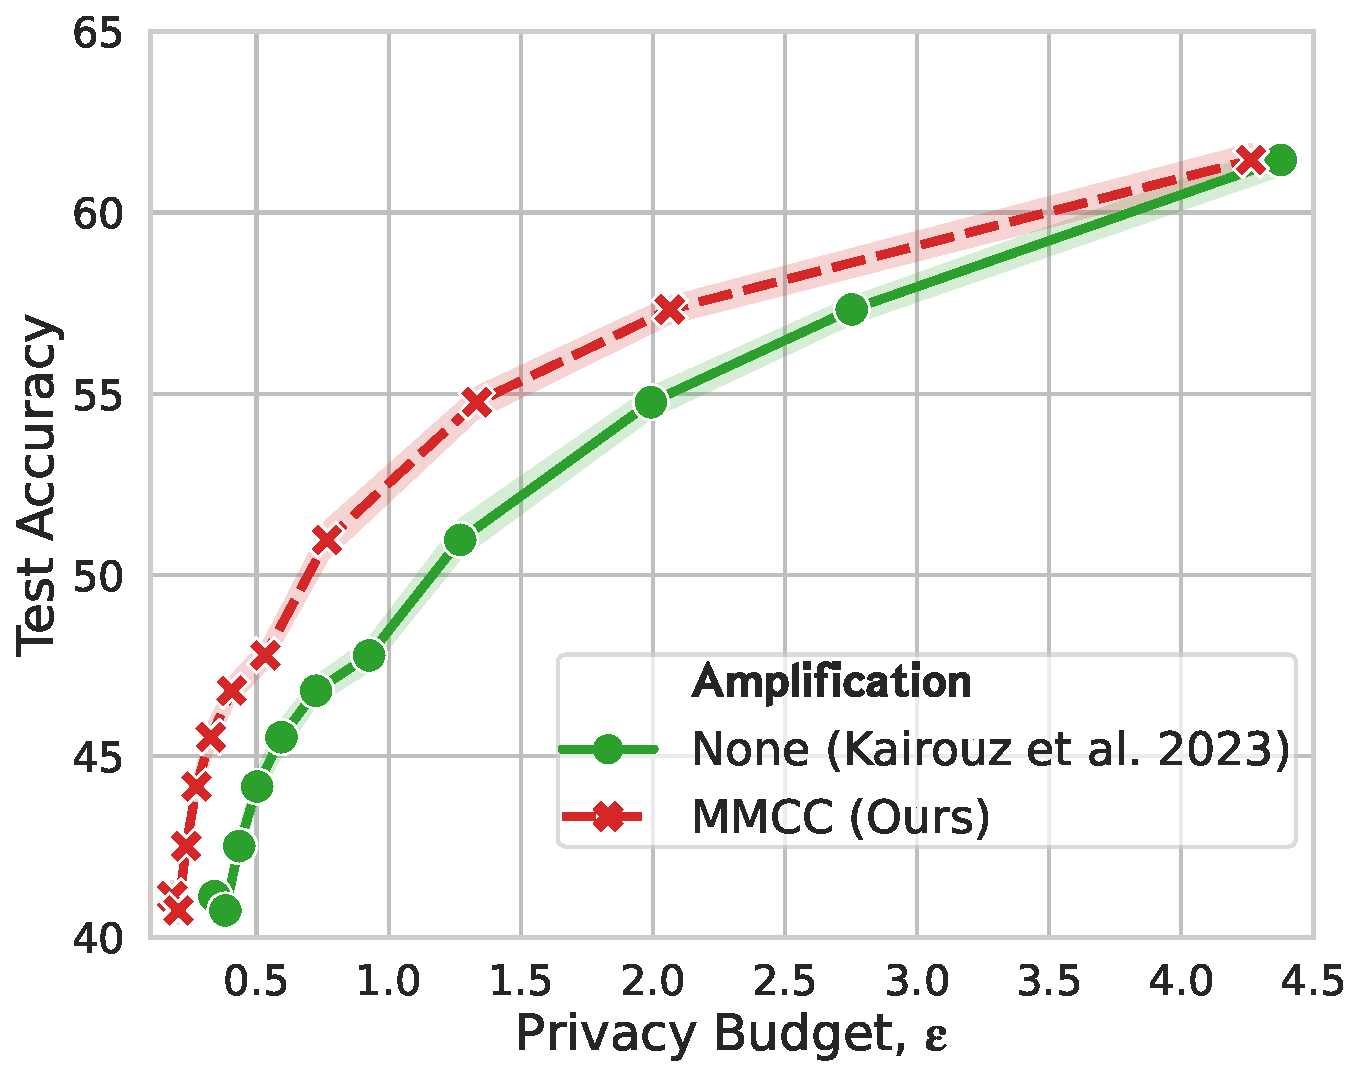
\includegraphics[width=0.7\textwidth]{plots/honaker_amplify.pdf}
    \caption{Our amplification analysis leads to significant gains over~\citet{kairouz2021practical} on practical ML experiments (CIFAR-10), entirely post-hoc.}
    \label{fig:improve-banded}
\end{minipage}\qquad
\begin{minipage}{.45\textwidth}
    \centering
    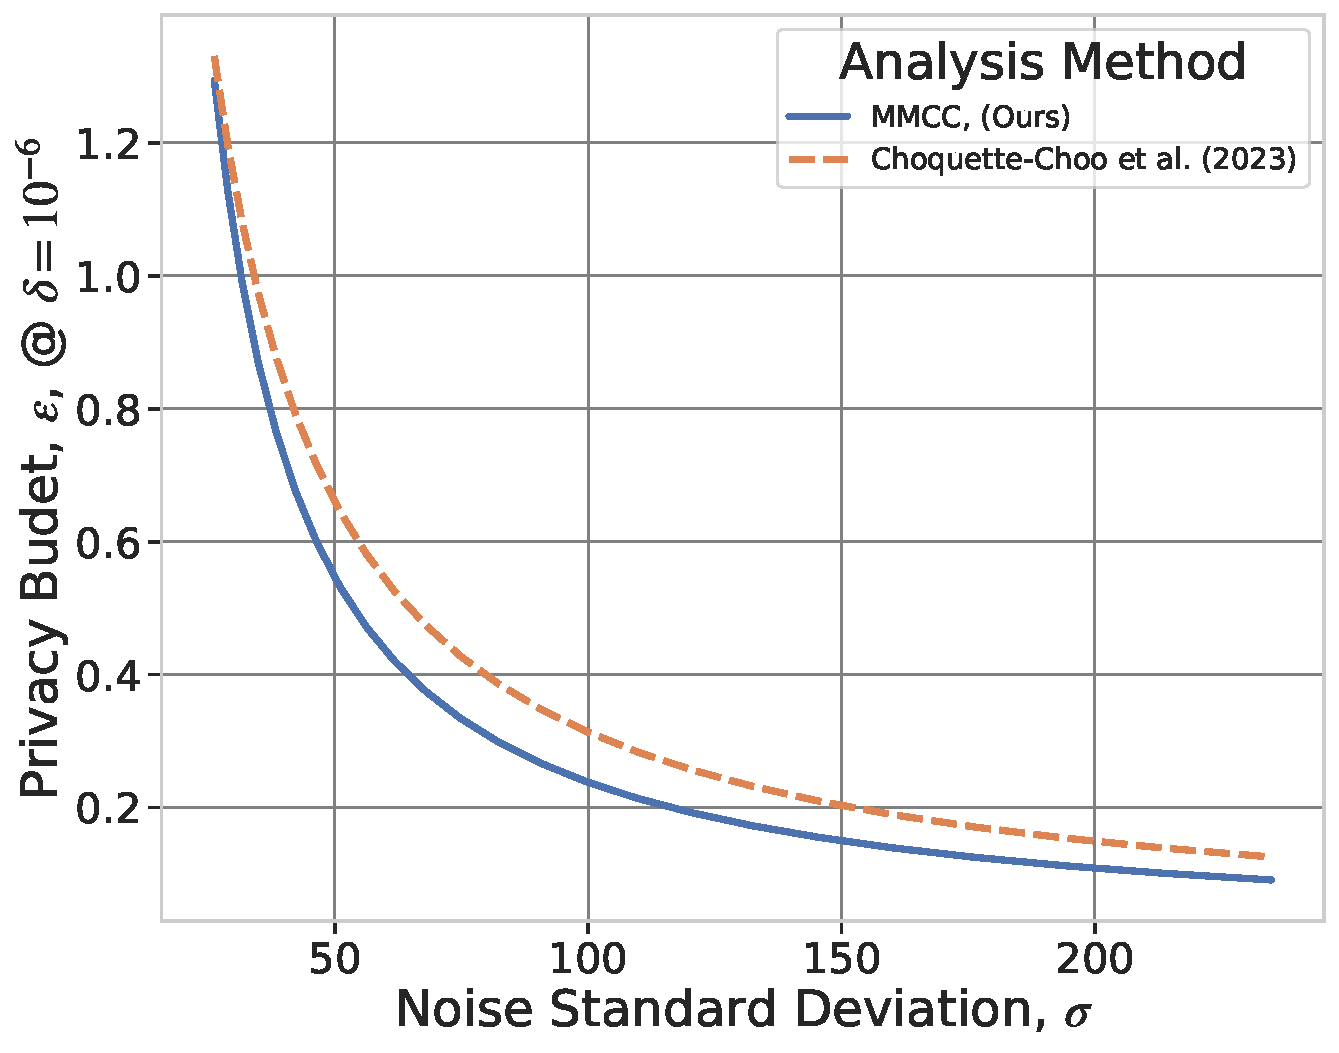
\includegraphics[width=.7\linewidth]{plots/eps_amplify_tree.pdf}
    \caption{\label{fig:tree-restart}\MMCC{} gives tighter $\epsilon$ than the analysis of \cite{BandedMF} for a DP-FTRL-TreeRestart mechanism of height $4$. Ran for $n=512$ steps with $p=\frac{1}{16}$.}
\end{minipage}
\end{figure}

\subsection{Correlated noise and amplification consistently beats independent noise}\label{sec:mse}

The prior work of \cite{BandedMF} gives an amplification result using a sampling scheme we call ``$b$-min-sep sampling'' for  $b$-banded matrices. In their sampling scheme, each example participates in $n/b$ rounds with sampling probability $bp$. In contrast, \MMCC{} enables sampling each example in all $n$ rounds with probability $p$, a ``more random'' form of sampling. We compare the two amplification analyses using the DP-FTRL-TreeRestart algorithm of \cite{kairouz2021practical}, which sequentially runs $n/2^{h-1}$ height-$h$ binary tree mechanisms, each binary tree mechanism run for $2^{h-1}$ rounds. This corresponds to a matrix mechanism that is $2^{h-1}$-banded, so we can apply the results of \cite{BandedMF}.
In \cref{fig:tree-restart}, we compare the $\epsilon$ for DP-FTRL-TreeRestart computed as a function of $\sigma$ using \MMCC{} and the analysis of \cite{BandedMF}, in the setting of $n = 512, p = 1/16, h = 4$, and we see that indeed the more random sampling enabled by \MMCC{} allows for improved privacy guarantees compared to $b$-min-sep sampling.